%	This LaTeX file is written by Zhiyang Ong for his presentation on instantaneous noise-based logic (iNBL).

%	The MIT License (MIT)

%	Copyright (c) <2016> <Zhiyang Ong>

%	Permission is hereby granted, free of charge, to any person obtaining a copy of this software and associated documentation files (the "Software"), to deal in the Software without restriction, including without limitation the rights to use, copy, modify, merge, publish, distribute, sublicense, and/or sell copies of the Software, and to permit persons to whom the Software is furnished to do so, subject to the following conditions:

%	The above copyright notice and this permission notice shall be included in all copies or substantial portions of the Software.

%	THE SOFTWARE IS PROVIDED "AS IS", WITHOUT WARRANTY OF ANY KIND, EXPRESS OR IMPLIED, INCLUDING BUT NOT LIMITED TO THE WARRANTIES OF MERCHANTABILITY, FITNESS FOR A PARTICULAR PURPOSE AND NONINFRINGEMENT. IN NO EVENT SHALL THE AUTHORS OR COPYRIGHT HOLDERS BE LIABLE FOR ANY CLAIM, DAMAGES OR OTHER LIABILITY, WHETHER IN AN ACTION OF CONTRACT, TORT OR OTHERWISE, ARISING FROM, OUT OF OR IN CONNECTION WITH THE SOFTWARE OR THE USE OR OTHER DEALINGS IN THE SOFTWARE.

%	Email address: echo "cukj -wb- 23wU4X5M589 TROJANS cqkH wiuz2y 0f Mw Stanford" | awk '{ sub("23wU4X5M589","F.d_c_b. ") sub("Stanford","d0mA1n"); print $5, $2, $8; for (i=1; i<=1; i++) print "6\b"; print $9, $7, $6 }' | sed y/kqcbuHwM62z/gnotrzadqmC/ | tr 'q' ' ' | tr -d [:cntrl:] | tr -d 'ir' | tr y "\n"



%%%%%%%%%%%%%%%%%%%%%%%%%%%%%%%%%%%%%%%%%%%%%%
%	Preamble

%	Acknowledgement:
%		This is based on a template provided to me by Dott. Francesco Stefanni, from the University of Verona in January 2011.
%
%	Number the slides per section. This makes it easier to track the index of the slides (or number of slides) per section, as opposed to the cumulative number of slides. When I manually track the number of slides for a presentation, each time I refactor the set of slides, I would have to update the slide numbers. I want the computer to do this automatically. Hence, I shall not do this manually.



%	Use the Beamer package to create the presentation slides.
\documentclass[xcolor={usenames,dvipsnames},hyperref={hyperindex,bookmarks}]{beamer}


%%%%%%%%%%%%%%%%%%%%%%%%%%%%%%%%%%%%%%%%%%%%%%
%	Import and Customize LaTeX packages.
\usepackage{beamerthemesplit}


%	Package for typesetting the following symbol: $\mathfrak{S}$
%\usepackage{amssymb}

%\mode<presentation>
%{ \usetheme{boxes} }

%	Select the presentation mode.
\mode<presentation>{
	\usetheme[logos=true,pagenumbers=true,background=true]{Esd}
}
\setbeamercovered{transparent}
%\setbeamercovered{invisible}


%	Import package to facilitate typesetting of algorithms.
\usepackage{listings}

\lstset{
  language=C++,
  tabsize=4,
%  basicstyle=\ttfamily\color{black}\small,
  basicstyle=\ttfamily\color{black},
%  backgroundcolor=\color{lightgray},
%  backgroundcolor=\color{white},
  keywordstyle=\color{Purple}\bfseries,
  identifierstyle=\color{OliveGreen},
  commentstyle=\color{Gray}\itshape,
  stringstyle=\color{CarnationPink},
  showstringspaces=false,
  showtabs=false,
  showspaces=false
}


\definecolor{lightgray}{gray}{0.95}
\font\emailtt=cmtt9

%	Set up configuration for hyperlinks.
%\usepackage[pdftex]{hyperref}	-- Option clash
\hypersetup{
    pdftitle={Programming Style for C},     % title
    pdfauthor={Francesco Stefanni},                 % author
    pdfsubject={A programming style for C}, % subject of the document
    pdfcreator={Creator},                           % creator of the document
    pdfproducer={dvipdft},                          % producer of the document
% Modified by Zhiyang Ong on Feb 7, 2011 to improve the way hyperlinks are colored in these presentation slides
	pdfkeywords={LaTeX, graphics, color},
%    pdfkeywords={C, C++, programming style},        % list of keywords
%
%    bookmarks=true,         % show bookmarks bar?
    unicode=false,          % non-Latin characters in Acrobats bookmarks
    pdftoolbar=true,        % show Acrobats toolbar?
    pdfmenubar=true,        % show Acrobats menu?
    pdffitwindow=false,     % window fit to page when opened
% Modified by Zhiyang Ong on Feb 7, 2011 to improve the way hyperlinks are colored in these presentation slides
	pdfpagemode=UseOutlines,bookmarks, bookmarksopen,
	pdfstartview=FitH, colorlinks, linkcolor=blue, citecolor=blue, urlcolor=red,
%    pdfstartview={Fit},    % fits the width of the page to the window
    pdfnewwindow=true,      % links in new window
% Modified by Zhiyang Ong on Feb 7, 2011 to improve the way hyperlinks are colored in these presentation slides
	colorlinks=red,        % false: boxed links; true: colored links
	linkcolor=red,          % color of internal links
%    colorlinks=false,        % false: boxed links; true: colored links
%    linkcolor=red,          % color of internal links
    citecolor=green,        % color of links to bibliography
    filecolor=magenta,      % color of file links
    urlcolor=red,           % color of external links
    pdfpagemode=FullScreen
    %
    %pdfpagelabels=false
}

%\usepackage[all]{hypcap}




%%%%%%%%%%%%%%%%%%%%%%%%%%%%%%%%%%%%%%%%%%%%%%
%	Added by Zhiyang Ong on Feb 7, 2011 to allow figures to be places side-by-side
%\usepackage{subfigure}









%%%%%%%%%%%%%%%%%%%%%%%%%%%%%%%%%%%%%%%%%%%%%%
%%%%%%%%%%%%%%%%%%%%%%%%%%%%%%%%%%%%%%%%%%%%%%
%%%%%%%%%%%%%%%%%%%%%%%%%%%%%%%%%%%%%%%%%%%%%%
%%%%%%%%%%%%%%%%%%%%%%%%%%%%%%%%%%%%%%%%%%%%%%
%%%%%%%%%%%%%%%%%%%%%%%%%%%%%%%%%%%%%%%%%%%%%%
%%%%%%%%%%%%%%%%%%%%%%%%%%%%%%%%%%%%%%%%%%%%%%
%%%%%%%%%%%%%%%%%%%%%%%%%%%%%%%%%%%%%%%%%%%%%%


%	Quantum Model Checking Is Not Evil: It Is Mandatory For Quantum Robots


%	First slide of the presentation
\title[Instantaneous Noise-Based Logic (iNBL)]
{\huge 
Instantaneous Noise-Based Logic}
\subtitle{My Work in Progress}
\author{Zhiyang Ong}
\institute{
	Department of Electrical and Computer Engineering \\
	Dwight Look College of Engineering,\\
	Texas A\&M University \\
	College Station, TX
}
\date{\today}	% (optional)
\subject{Subject Title}

%	This set of presentation slides is based on \cite{Ying2014a}, from my BibTeX research database.







%%%%%%%%%%%%%%%%%%%%%%%%%%%%%%%%%%%%%%%%%%%%%%
%	Do nothing in this section of the LaTeX document

\begin{document}

\begin{frame}
\titlepage
\end{frame}



%	%	Table of Contents
%	\AtBeginSection[]		% Do nothing for \subsection*
%	{
%		\begin{frame}
%	%		\frametitle{\textcolor{yellow}{Table of Contents}}
%			\frametitle{Table of Contents}
%	%		\textcolor{yellow}{\tableofcontents[currentsection]}
%			\tableofcontents[currentsection,currentsubsection]
%		\end{frame}
%	}
%	
%	\AtBeginSubsection[]		% Do nothing for \subsection*
%	{
%	\begin{frame}
%	\tableofcontents[currentsection,currentsubsection]
%	\end{frame}
%	}
%	
%	\section*{Outline}
%	\begin{frame}
%	\tableofcontents
%	\end{frame}



%%%%%%%%%%%%%%%%%%%%%%%%%%%%%%%%%%%%%%%%%%%%%%
%
%	Slides begin HERE!!!
%
%%%%%%%%%%%%%%%%%%%%%%%%%%%%%%%%%%%%%%%%%%%%%%


%%%%%%%%%%%%%%%%%%%%%%%%%%%%%%%%%%%%%%%%%%%%%%
%	Preamble

%	Slide #1
\frame
{
	\frametitle{Cheap(er), Small(er), and Fast(er)!!!}
	\framesubtitle{Is that possible? For real???}

	\begin{columns}[t]			% Contents are top vertically aligned
		\begin{column}[T]{5cm}	% Each column can also be its own environment
		
		More Moore's Law, Generalized Moore's Law, More than Moore's Law \\
		\ \\
		Continuum Noise-Based Logic (NBL): %\vspace{-0.2cm}
		\begin{itemize} %\itemsep -2pt
		\item Deterministic
		\item Reduce error accumulation \&\ propagation
		\item More energy efficient
		\item Greater circuit complexity
		\end{itemize}
%Deterministic (non-probabilistic)
		\end{column}
		
		\begin{column}[T]{5cm}	% Alternative top-align that's better for graphics
			\begin{figure}
			\centering
			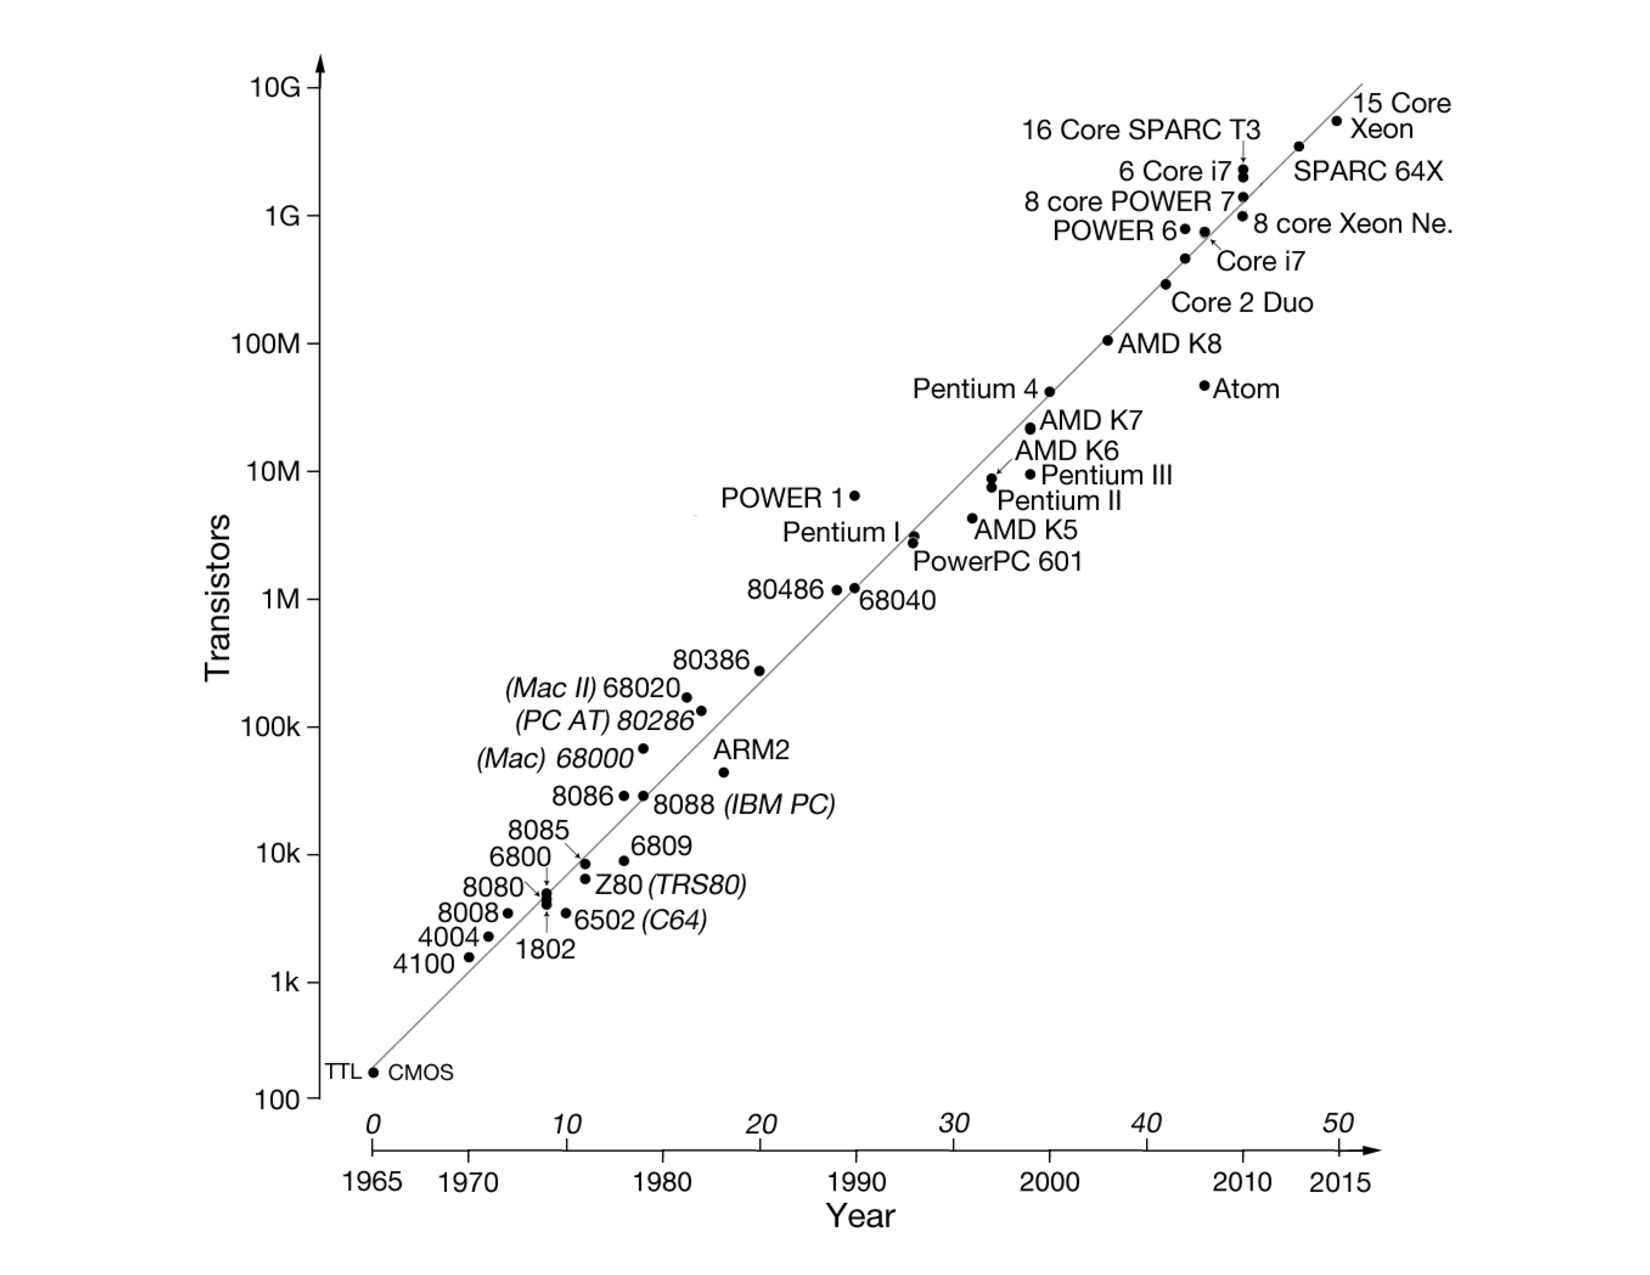
\includegraphics[height=1.8in]{./pics/moores_law_2015}
			%\caption{Semi-log Plot (log-lin type) of the number of transistors on a processor against time. Reference: \url{https://www.elektormagazine.com/articles/moores-law}}
			\caption{Semi-log Plot (log-lin type) of the number of transistors on a processor against time.}
			\end{figure}
		\end{column}
	\end{columns}
}

%	Reference: https://www.elektormagazine.com/articles/moores-law
\begin{frame}
	\frametitle{Noise-Based Logic (NBL)}
%	\framesubtitle{Slide Subtitle 5.}
	
	\begin{figure}
		\centering
		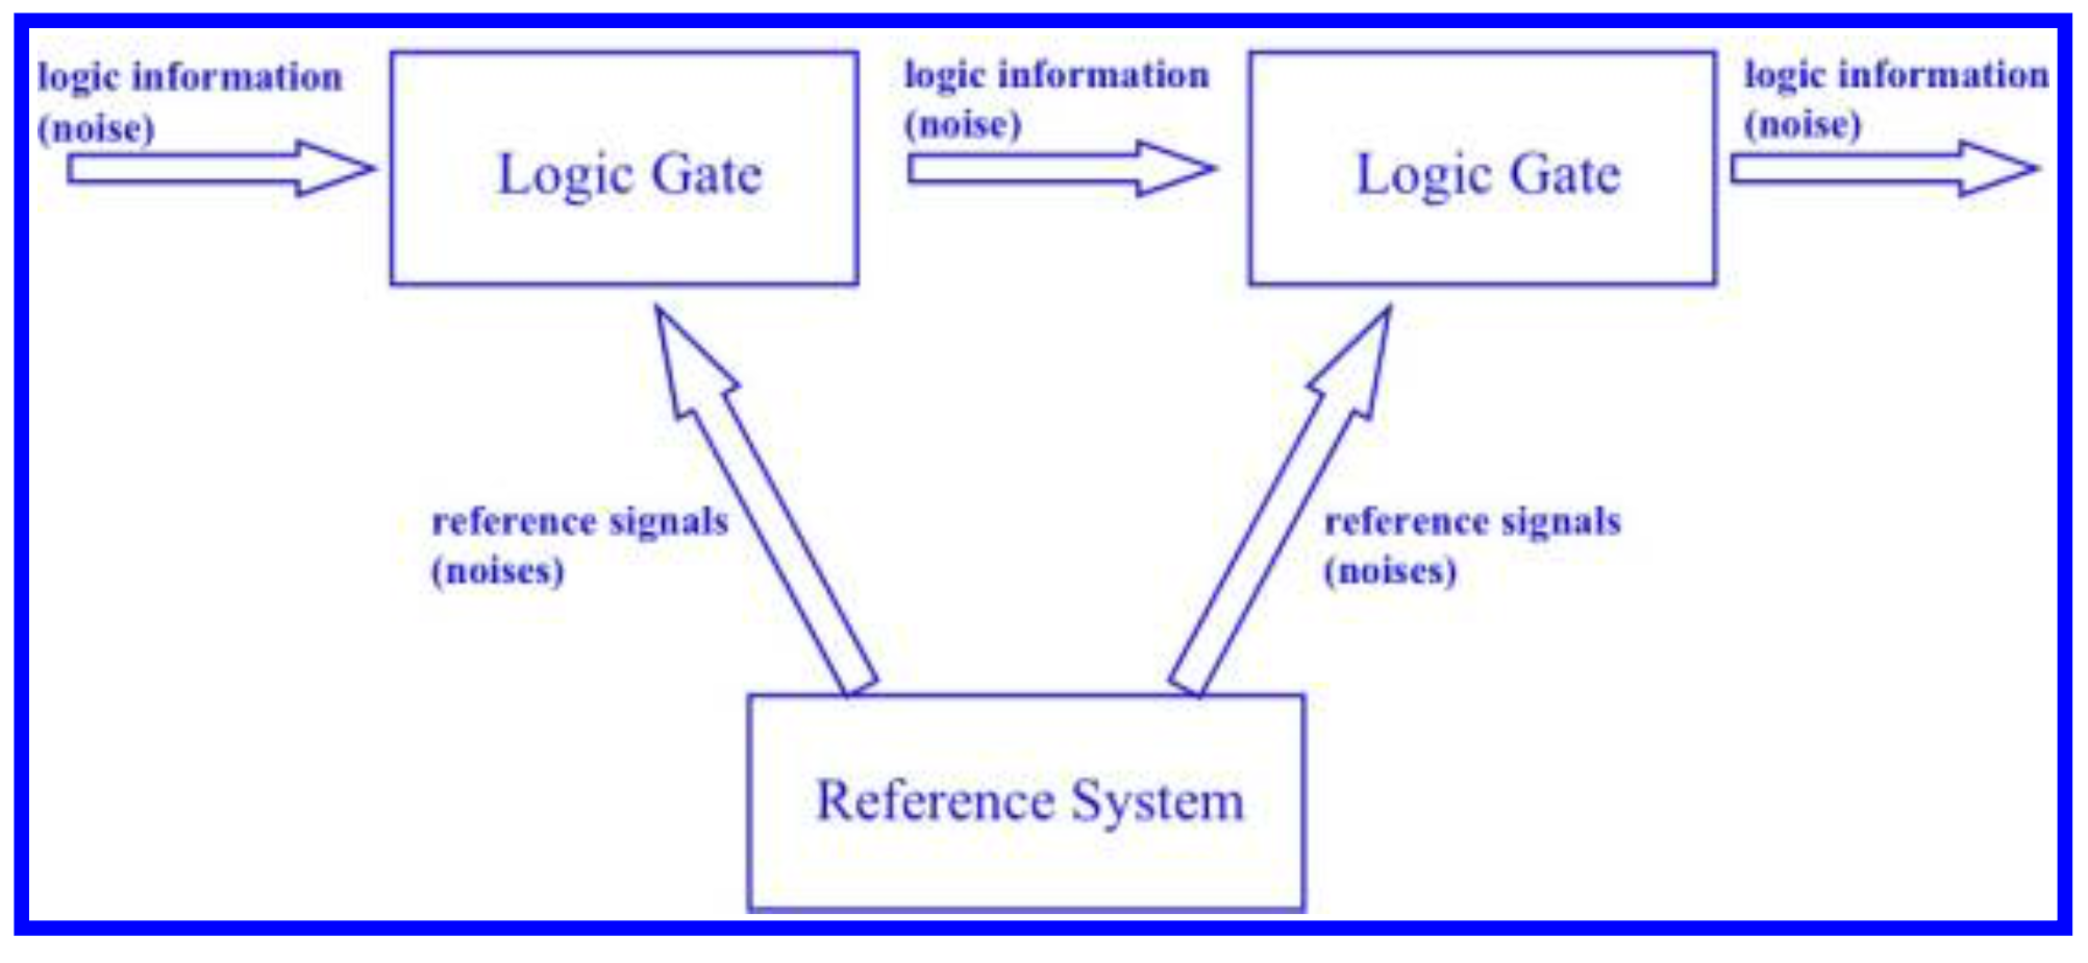
\includegraphics[height=2in]{./pics/generic_nbl}
		\caption{Generic framework for Noise-Based Logic (NBL).}
	\end{figure}
\end{frame}


\begin{frame}
	\frametitle{Design implementations of continuum NBL}
%	\framesubtitle{Slide Subtitle 5.}
	
	\begin{figure}
		\centering
		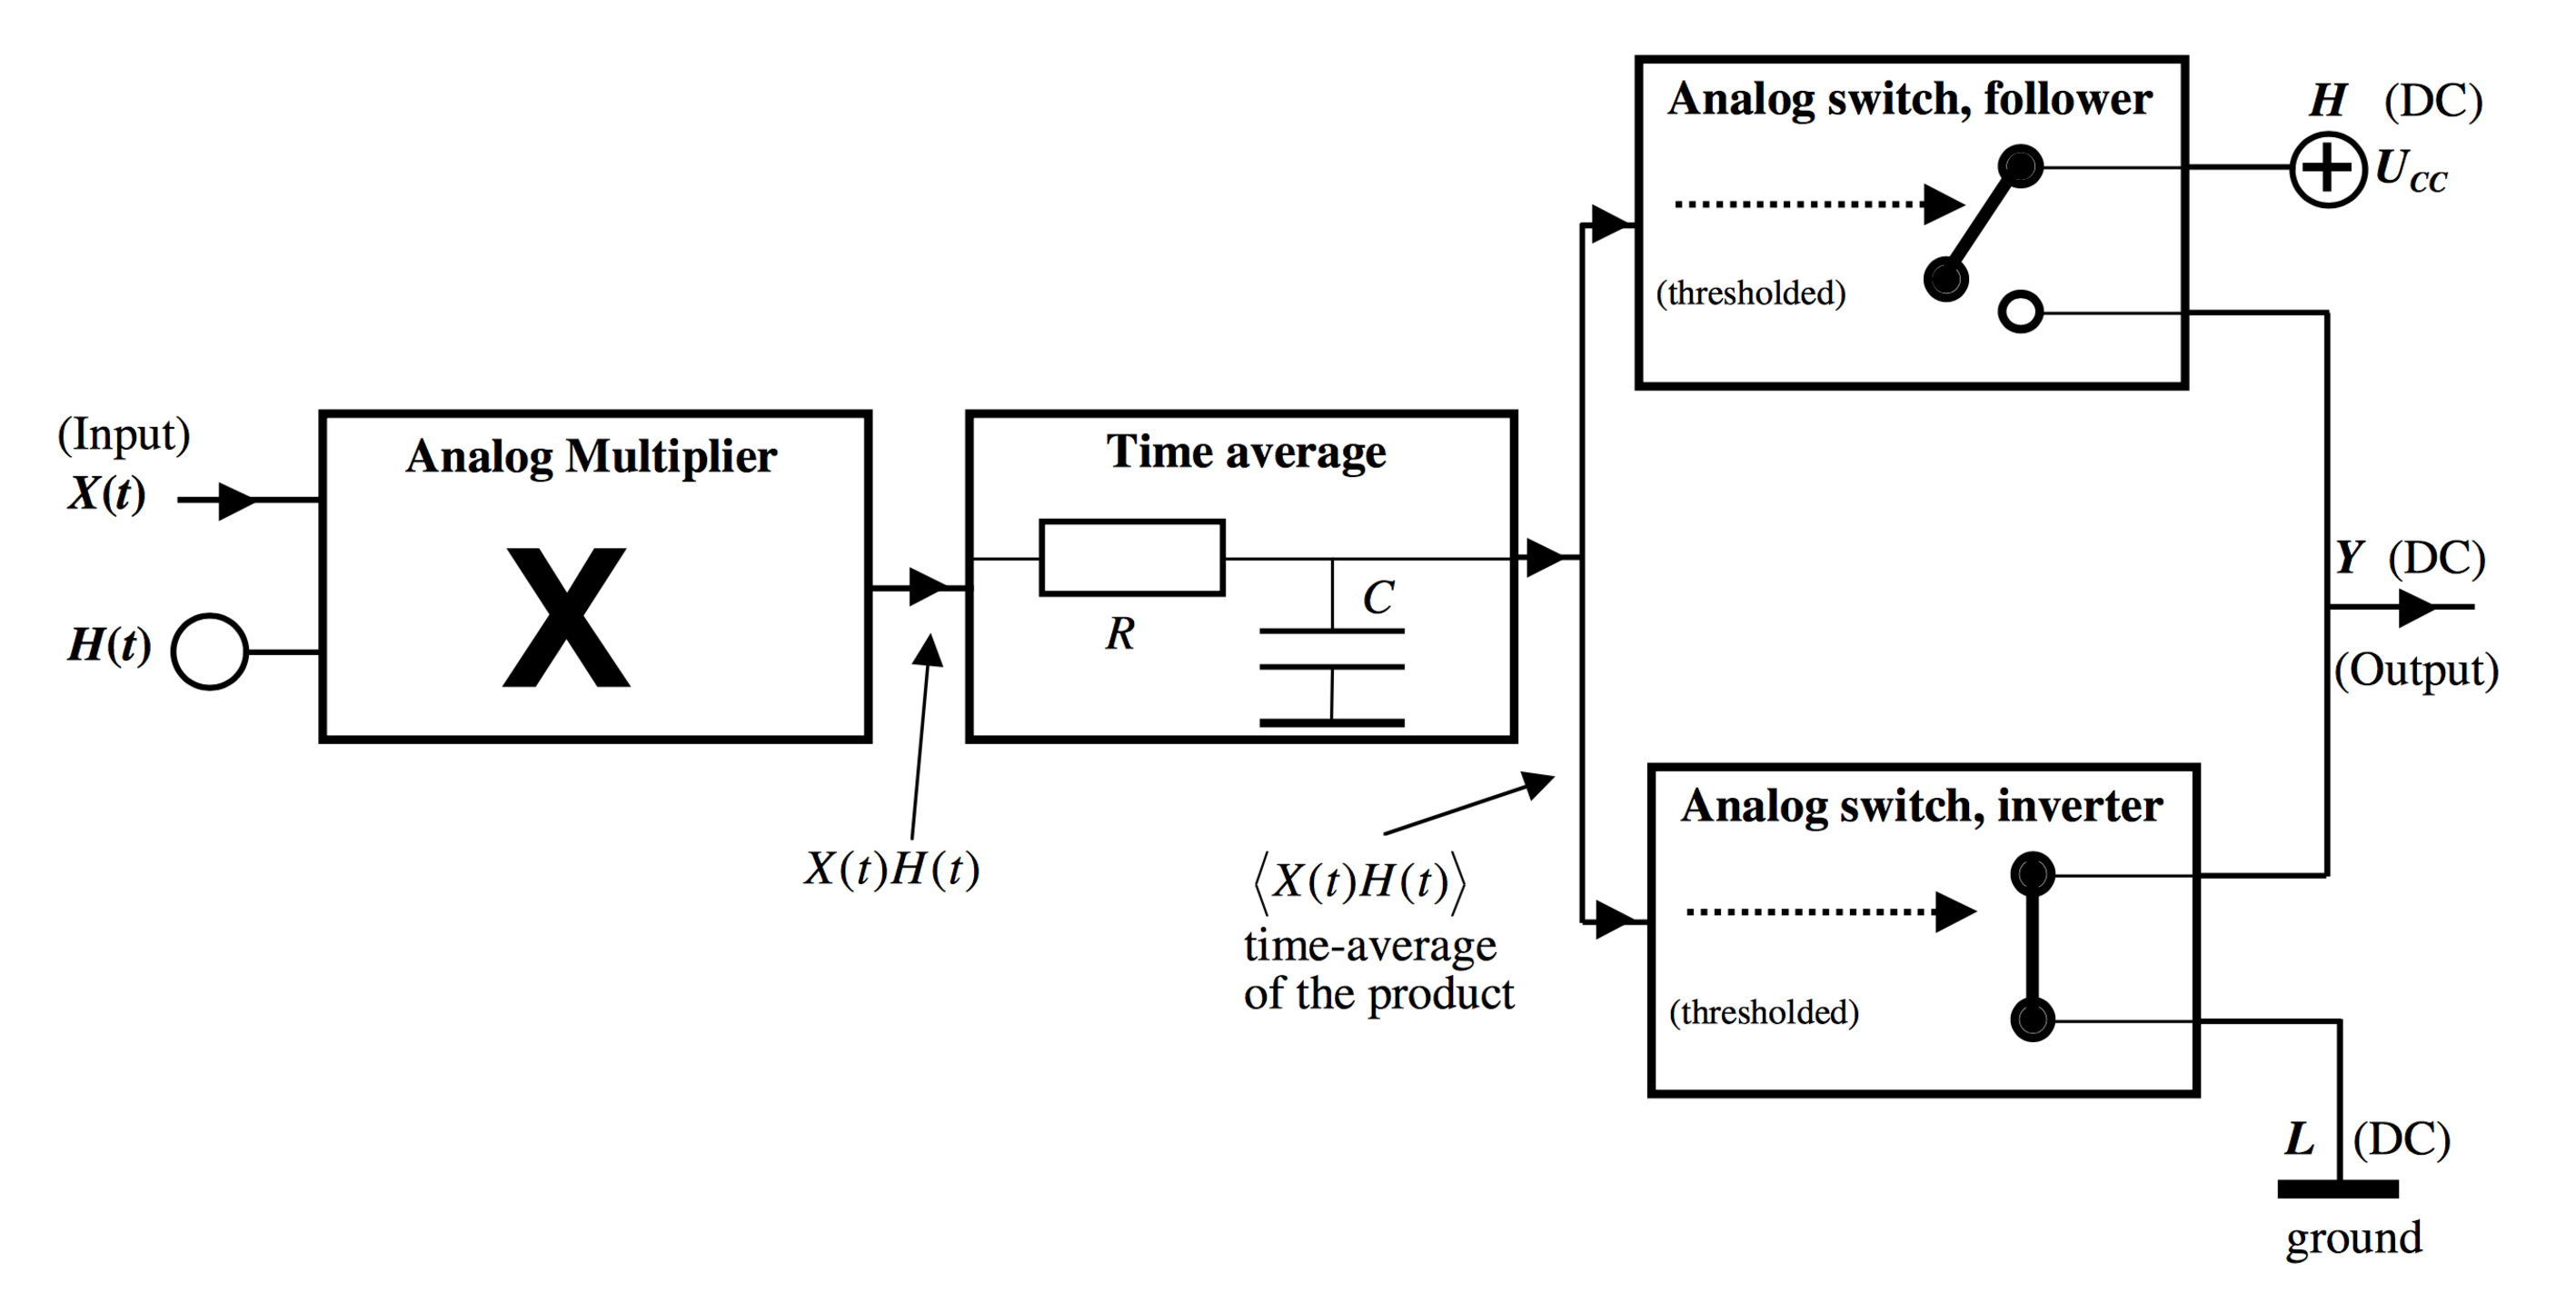
\includegraphics[height=2in]{./pics/continuum_nbl}
		\caption{Schematic for the {\tt FOLLOWER} gate in continuum NBL.}
	\end{figure}
\end{frame}




%%%%%%%%%%%%%%%%%%%%%%%%%%%%%%%%%%%%%%%%%%%%%%
%	Instantaneous Noise-Based Logic (iNBL)
\section{Instantaneous Noise-Based Logic (iNBL)}

%	Slide 1
\frame
{
	\frametitle{Instantaneous Noise-Based Logic (iNBL)}

	iNBL: no time averaging operations, with the exception of the output interfaces. \\
	\ \\
	$\therefore$ NBL schemes without time averaging are instantaenous. \\
	\ \\
	\begin{itemize}
	\item Advantages over continuum NBL: %\vspace{-0.3cm}
		\begin{itemize} %\itemsep -2pt
		\item Performance (computational time complexity) speedup by 10-100 X.
		\item Simpler, hence cheaper, circuit complexity.
		\end{itemize}
	\item Examples of iNBL schemes:
		\begin{itemize}
		\item noise-based brain logic scheme
		\item bipolar random telegraph waves
		\end{itemize}
	\end{itemize}
}



%	Slide 2
\frame
{
	\frametitle{Bipolar Random Telegraph Waves (bipolar RTW)}

	Bipolar random telegraph waves (RTW) is defined by the function {\tt bipolar\_rtw(n)}. \
	\ \\
	\begin{gather*}
	{\tt bipolar\_rtw(n)} =
		\begin{cases}
		1, & {\tt random(n)} \geq 0.5, \\
		-1, & {\tt random(n)} < 0.5,
		\end{cases}
		\ \\
	\forall n \in \{1, 2, 3, \dots\} ({\rm or\ n} \in |\mathbb{Z}| > 0)
	\end{gather*}
	where $n$ is the $n^{th}$ time step in a bipolar logic signal, {\tt bipolar\_rtw(n)} $\in \{1, -1\}$, that is generated from a (pseudo-) random noise generator. 
}



\begin{frame}
	\frametitle{Bipolar RTW Signals}
%	\framesubtitle{Slide Subtitle 5.}
	
	\begin{figure}
		\centering
		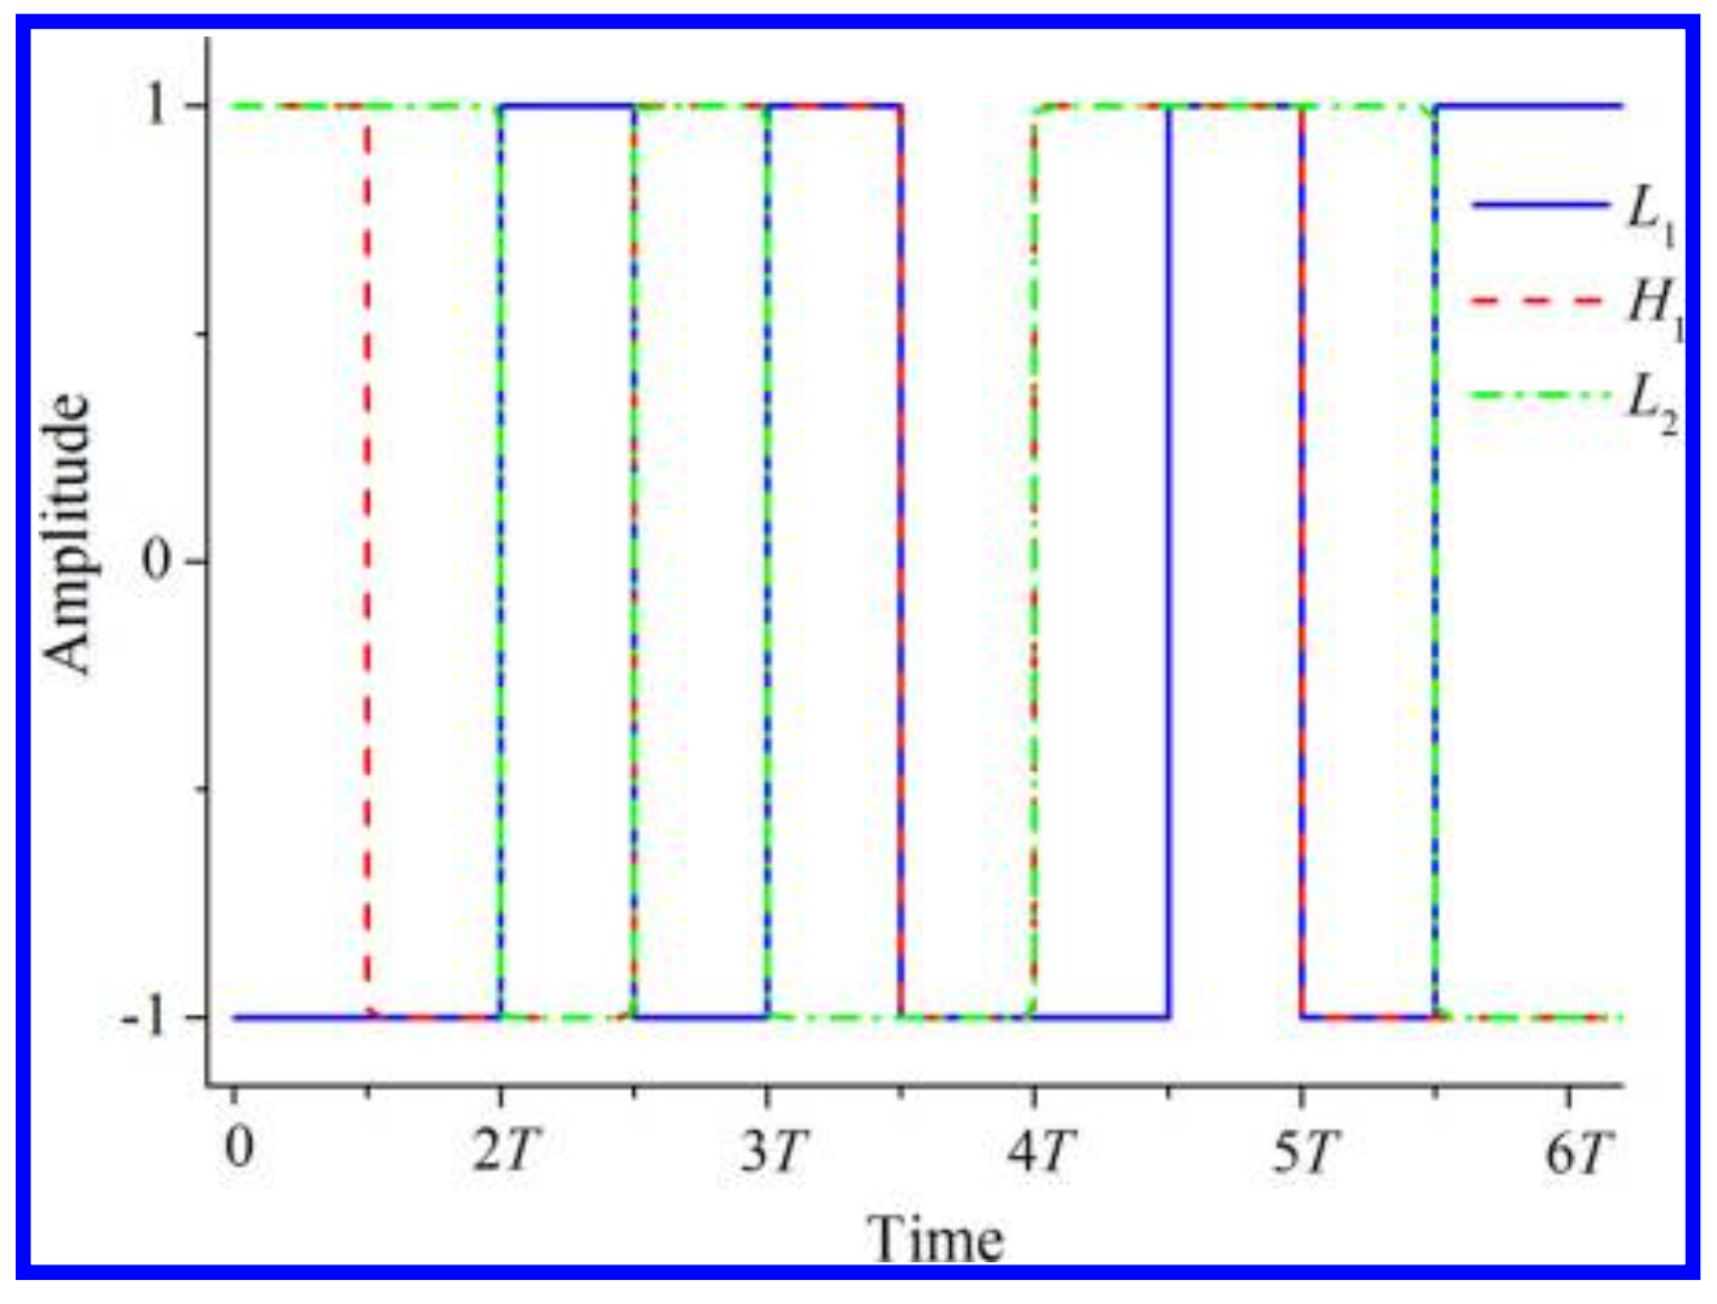
\includegraphics[height=2.6in]{./pics/inbl}
		\caption{Sample bipolar RTW signal for iNBL.}
	\end{figure}
\end{frame}


\begin{frame}
	\frametitle{Time-Shifted Bipolar RTW Signals}
%	\framesubtitle{Slide Subtitle 5.}
	
	\begin{figure}
		\centering
		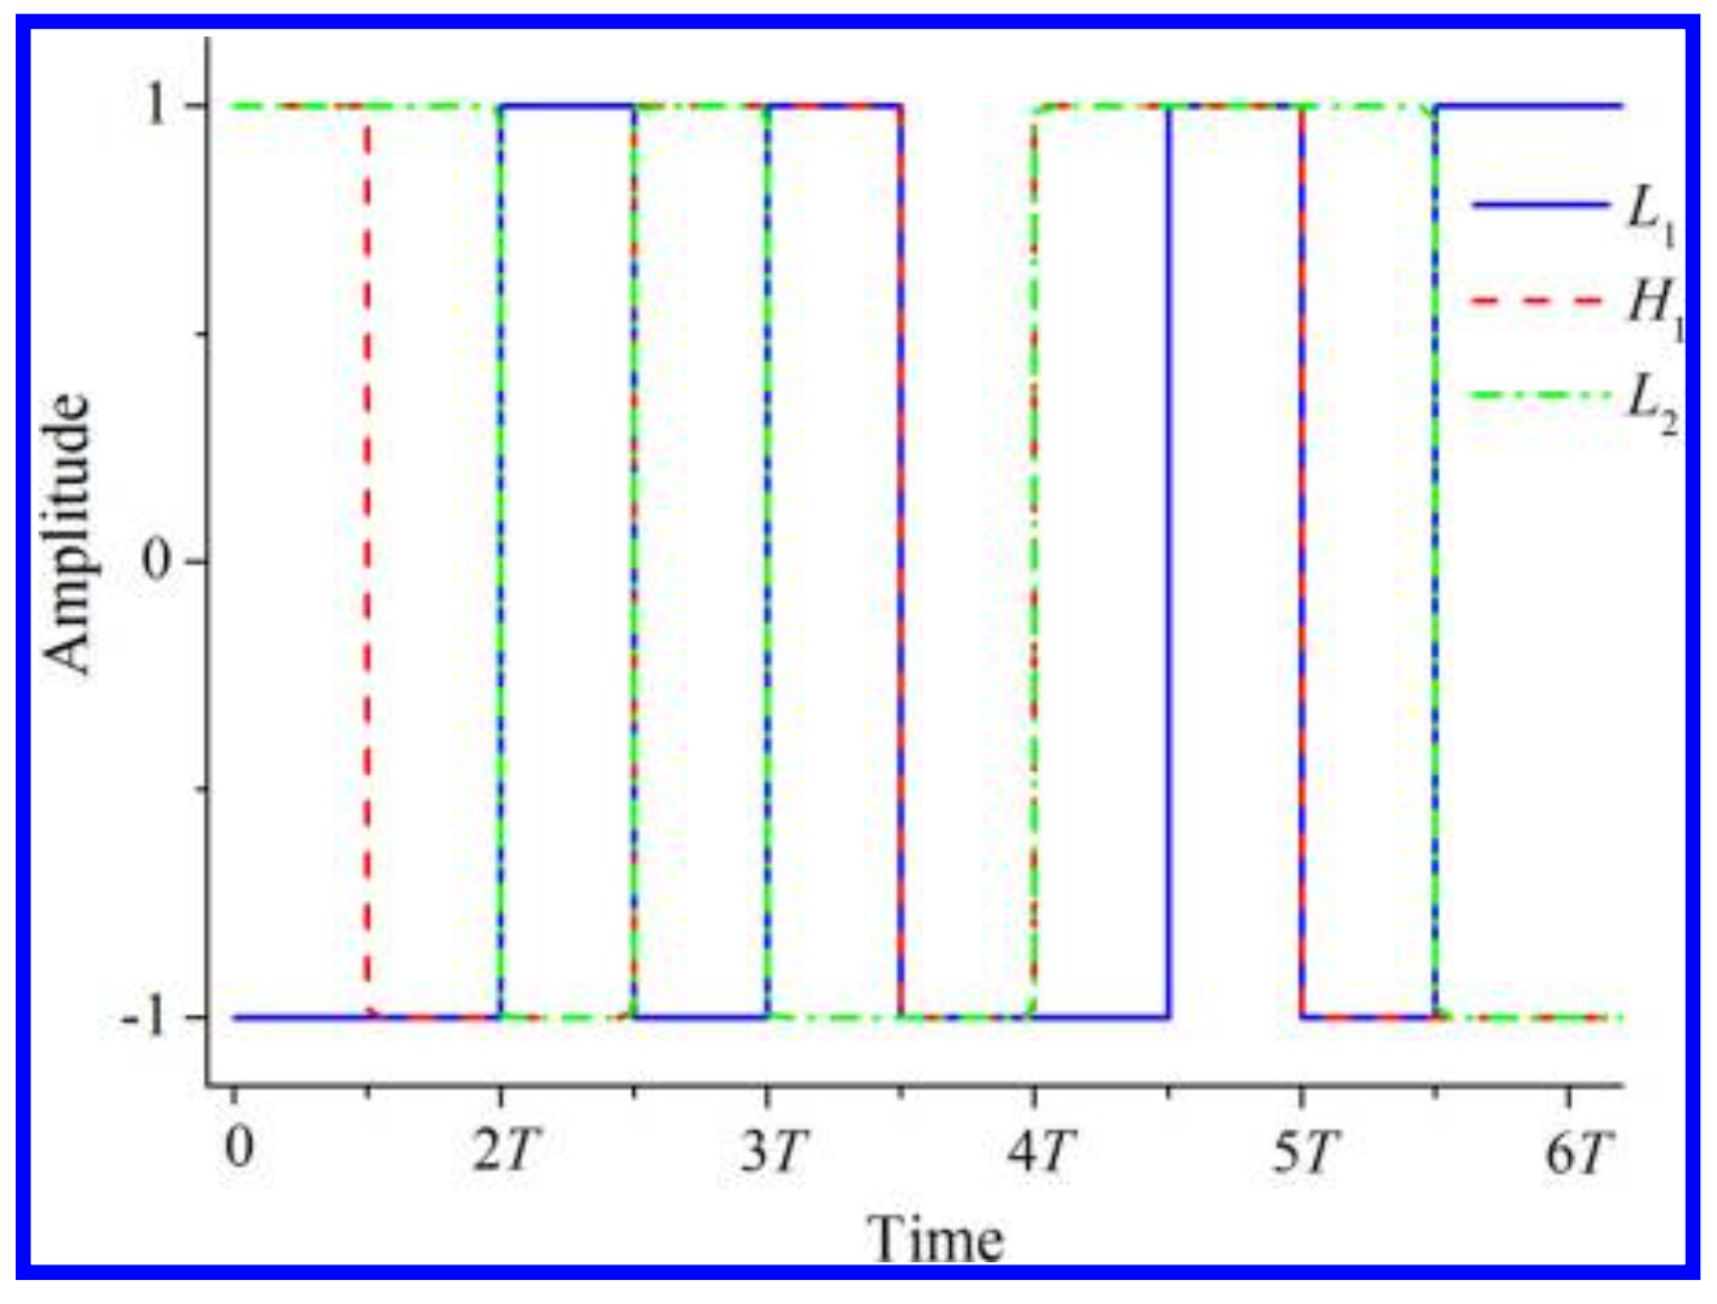
\includegraphics[height=2.6in]{./pics/inbl}
		\caption{Sample time-shifted bipolar RTW signal for time-shifted iNBL (TSINBL).}
	\end{figure}
\end{frame}


%	Slide 3
\frame
{
	\frametitle{References for Classical Reachability Analysis}

	(Yuan, 2006) Yuan, J., Pixley, C., and Aziz, A. Constrained-Based Verification. Springer Science+Business Media, Inc., New York, NY, 2006.
}








%%%%%%%%%%%%%%%%%%%%%%%%%%%%%%%%%%%%%%%%%%%%%%
%	Problem Statement
\section{Problem Statement}


%	Slide 2
\frame
{
	\frametitle{Problem Statement}

	\begin{itemize} %\itemsep -2pt
	\item Models of concurrent and nondeterministic quantum systems need to be verified.
	\item Quantum Markov decision processes (qMDPs) can model such quantum systems.
	\item Question: How can we carry out reachability analysis on concurrent and nondeterministic quantum systems, modeled as qMDPs?
	\item Input: qMDP $\mathcal{M}$
	\item Input: state space $\mathcal{H}$, which is a Hilbert space
	\item Input: state space $B \in \mathcal{H}$
	\item Output: Scheduler $\mathfrak{S}$
	\item Output: Non-negative integer, $n$.
%	\item Input: Description of system behavior
%		\begin{itemize}
%		\item i.e., specifications based on quantum automata
%		\end{itemize}
%	\item Input: Functional linear-time properties
%		\begin{itemize}
%		\item Linear-time invariants of quantum automata-based model
%		\end{itemize}
	%\item System model based on quantum automata
	%\item System propeties (i.e., invariants): invariants of quantum automata-based model.
	%\item Output: Boolean flag indicating correct/incorrect system behavior/functionality
	\end{itemize}
}




%	Slide 3
\frame
{
	\frametitle{Shortcomings of Classical Reachability Analysis}

	\begin{itemize} %\itemsep -3pt
	\item Classic Markov chains cannot capture concurrency.
	\item A Markov chain only allows one ``choice'' of action per state, which implies that all ``rewards'' of the Markov chain are the same.
	\item Cannot formalize behavior/functionality of quantum systems
		\begin{itemize}
		\item Discrete state spaces of classical systems are finite or countably finite
		\item Continuous state spaces of quantum systems cannot be addressed by discrete state spaces
		\item State spaces of quantum systems are continuous, even for finite-dimensional quantum systems
		\item Need to examine a finite number of representative elements  (in an orthonormal basis) of the state space of a quantum system
		\item Or, at most, examine countably infinitely many representative elements of this state space
		\item Always preserve the linear algebraic structure of the representative elements [\& linear-time properties]
		\end{itemize}
	\item Cannot formally describe temporal properties of quantum systems
	\item The (Ying 2014) paper address quantum programs. However, the modeling of quantum programs can be extended for quantum systems, including quantum robots?
	\end{itemize}
}









%%%%%%%%%%%%%%%%%%%%%%%%%%%%%%%%%%%%%%%%%%%%%%
%	Prior Works
\section{Prior and Related Works}

%	Slide 4
\frame
{
	\frametitle{Prior and Related Work}

	\begin{itemize}
	\item Almost all previous work use model checking to verify quantum communication protocols
	\item Use quantum process algebra to verify quantum communication systems, including quantum error correction codes
	\item Use simulation tools for quantum systems to verify their behavior/functionality, especially their correctness and safety properties
	\item Quantum partially observable Markov decision processes (QOMDPs), which are introduced by (Barry, Barry, and Aaronson, 2014), only care about the reachability of a single state (i.e., goal state).: %\vspace{-0.2cm}
		\begin{itemize} \itemsep -2pt
		\item The paper does not specifically address the reachability of invariant subspaces.
		\item Goal-state reachability is undecidable for QOMDPs.
		\end{itemize}
	\end{itemize}
}


Invariant subspace: sounds like T: V-->V
something that transforms you into the same space







%%%%%%%%%%%%%%%%%%%%%%%%%%%%%%%%%%%%%%%%%%%%%%
%	Design Decisions
\section{Design Decisions}

%	Slide 5
\frame
{
	\frametitle{Design Decisions}

	\begin{itemize}
	\item Quantum model checking framework for the formal verification of generic quantum engineering systems
		\begin{itemize}
		\item Not just quantum communication systems
		\end{itemize}
	\item Use a formal method based on modeling quantum systems with quantum automaton
		\begin{itemize}
		\item Exploit similar work in quantum Markov chains, quantum dot automata, \& quantum cellular automata
		\end{itemize}
	\item Only consider linear-time properties of generic quantum systems
		\begin{itemize}
		\item Describe these linear-time properties as infinite sequences of sets of atomic propositions, just like LTL model checking
		\end{itemize}
	\item Extend this to verify safety properties for reversible automata
	\item Extend this to verify $\omega$-properties for reversible B{\"{u}}chi automata
	\item Meet requirements for correctness, safety, \&\ reliability
	\end{itemize}
}











%%%%%%%%%%%%%%%%%%%%%%%%%%%%%%%%%%%%%%%%%%%%%%
%	Key Contributions of Ying2014a
\section{Key Contributions of (Ying 2014)}

%	Slide 6
\frame
{
	\frametitle{Key Contributions of (Ying 2014)}

	\begin{itemize}
	\item 
	\end{itemize}
}











%%%%%%%%%%%%%%%%%%%%%%%%%%%%%%%%%%%%%%%%%%%%%%

%\section{Background Information}

%\subsection{Background Information}
%
%\frame
%{
%	\frametitle{Coursework Related to Electronic Design Automation}
%
%	\begin{itemize}
%	\item<1-> University of Southern California: \vspace{-0.05cm}
%		\begin{itemize} \itemsep -1pt
%		\item Electronic Design Automation + Digital VLSI Testing: \vspace{-0.1cm}
%			\begin{itemize} \itemsep -1pt
%			\item EE 680 -- Computer Aided Design of Digital Systems I
%			\item EE 599/581 -- Mathematical Foundations for Computer Aided Design of VLSI Systems
%			\item EE 658 -- Diagnosis and Design of Reliable Digital Systems
%			\end{itemize}
%		\item Digital VLSI Design: \vspace{-0.1cm}
%			\begin{itemize} \itemsep -1pt
%			\item EE 477L -- MOS VLSI Circuit Design
%			\item EE 577A/B -- VLSI System Design
%			\end{itemize}
%		\end{itemize}
%	\item<2-> University of Adelaide: \vspace{-0.05cm}
%		\begin{itemize} \itemsep -1pt
%		\item Introductory Digital VLSI Design: \vspace{-0.1cm}
%			\begin{itemize} \itemsep -1pt
%			\item Elec Eng 4037 -- Digital Microelectronics
%			\item Elec Eng 3017 -- Digital Electronics
%			\end{itemize}
%		\item Software Engineering: \vspace{-0.1cm}
%			\begin{itemize} \itemsep -1pt
%			\item Comp Sci 3006 -- Software Engineering and Project
%			\end{itemize}
%		\item Relevant classes for my research topic: \vspace{-0.1cm}
%			\begin{itemize} \itemsep -1pt
%			%\item Elec Eng 4044 -- RF Engineering IV
%			%\item Elec Eng 3021 -- Electrical Energy Systems
%			%\item Elec Eng 4042 -- Power Electronics and Drive Systems
%			\item Elec Eng 3015 -- Communications, Signals, \& Systems
%			\item Elec Eng 3016 -- Control III
%			\item Elec Eng 3018 -- RF Engineering III
%			%\item Elec Eng 3020 -- Embedded Computer Systems
%			\end{itemize}
%		\end{itemize}
%	\end{itemize}
%}









%%%%%%%%%%%%%%%%%%%%%%%%%%%%%%%%%%%%%%%%%%%%%%

%\section{Research and Project Experience}
%
%\subsection{Problem Description}
%
%\frame
%{
%	\frametitle{Research Background}
%
%	\begin{itemize}
%	\item<1-> Literature Review: \vspace{-0.05cm}
%		\begin{itemize} \itemsep -1pt
%		\item Robotic Surgery + Biomedical MEMS
%		\end{itemize}
%	\item<2-> Honors research project / Senior thesis: \vspace{-0.05cm}
%		\begin{itemize} \itemsep -1pt
%		\item Complex Systems + Evolutionary Computation
%		\end{itemize}
%	\item<3-> Masters Research Project: \vspace{-0.05cm}
%		\begin{itemize} \itemsep -1pt
%		\item Automatic Test Pattern Generation at Electronic System-Level�(Attempted)
%		\item Computer System Performance Analysis (vertical profiling)
%		\end{itemize}
%	\end{itemize}
%}


%%%%%%%%%%%%%%%%%%%%%%%%%%%%%%%%%%%%%%%%%%%%%%

%\section{Research and Project Experience}

%\subsection{Project Experience}
%
%\frame
%{
%	\frametitle{Project Experience}
%
%	\begin{itemize}
%	\item<1-> EDA Software Development: \vspace{-0.05cm}
%		\begin{itemize} \itemsep -1pt
%		\item ATPG for FPGA test generation system
%		\item C++ Parser for IEEE STIL format
%		\item Gate-level logic simulator for combinational VLSI circuits
%		\item Software for crosstalk-aware gate sizing in VLSI circuits
%		\end{itemize}
%	\item<2-> Digital VLSI Design: \vspace{-0.05cm}
%		\begin{itemize} \itemsep -1pt
%		\item Viterbi decoder
%		\item 32-kbit synchronous SRAM with 32-bit words
%		\item 64-bit Ladner-Fischer tree adder
%		\item 32-bit variable length carry-increment adder
%		\end{itemize}
%	\item<3-> Processor Design: \vspace{-0.05cm}
%		\begin{itemize} \itemsep -1pt
%		\item 4-stage pipelined Troy Wideword Processor (128-bit datapath)
%		\item 32-bit MIPS processor (multi-cycle \& pipeline implementations)
%		\item AMD Am2901 microprocessor
%		\end{itemize}
%	\end{itemize}
%}






%%%%%%%%%%%%%%%%%%%%%%%%%%%%%%%%%%%%%%%%%%%%%%

\section{Analysis on Decidability of Quantum Reachability Analysis}

%%%%%%%%%%%%%%%%%%
%\subsection{In the Finite-Horizon}

%	Slide #1
\frame
{
	\frametitle{Analysis on Decidability of Quantum Reachability Analysis In the Finite-Horizon}

	\begin{itemize}
	\item 
	\end{itemize}
}








%%%%%%%%%%%%%%%%%%
%\subsection{In the Infinite-Horizon}

%	Slide #1
\frame
{
	\frametitle{Analysis on Decidability of Quantum Reachability Analysis In the Infinite-Horizon}

	\begin{itemize}
	\item 
	\end{itemize}
}






%%%%%%%%%%%%%%%%%%%%%%%%%%%%%%%%%%%%%%%%%%%%%%

\section{Analysis on Complexity of Quantum Reachability Analysis}

%%%%%%%%%%%%%%%%%%
%\subsection{In the Finite-Horizon}

%	Slide #1
\frame
{
	\frametitle{Analysis on Complexity of Quantum Reachability Analysis In the Finite-Horizon}

	\begin{itemize}
	\item 
	\end{itemize}
}








%%%%%%%%%%%%%%%%%%
%\subsection{In the Infinite-Horizon}

%	Slide #1
\frame
{
	\frametitle{Analysis on Complexity of Quantum Reachability Analysis In the Infinite-Horizon}

	\begin{itemize}
	\item 
	\end{itemize}
}





%%%%%%%%%%%%%%%%%%%%%%%%%%%%%%%%%%%%%%%%%%%%%%

\section{Questions That I Have}

%\subsection{Yet to be defined}


%	Slide #1
\frame
{
	\frametitle{Questions That I Have}

	\begin{itemize}
	\item I assume that uncomputable problems are the same as undecidable problems (Barry, Barry, and Aaronson, 2014). %Is this actually true?
	\item From (Barry, Barry, and Aaronson, 2014), can QOMDPs be reduced to qMDPs?
	\item The authors mentioned that quantum systems can be modeled as qMDPs? Do such quantum systems include robots, which can be modeled as quantum dynamical systems? Or, is it restricted to quantum computer programs?
	\item What is the ortho-complement of a subspace?
%	See page 2, left column, in the middle of the 3rd/4th paragraph that starts with the following in bold, "Contribution of the paper".
	\item What does it mean for a measurement to be projective? What does it mean mathematically?
%	Page 2, right column, in the 2nd/3rd paragraph. 
	\item Is ``W'' on page 2, right column, in the last paragraph ($w \in W$), a set of words ``w''?
	\item $\otimes$, right column, in paragraph 1/2 on page 2
	\end{itemize}
}

do Markov chains inherently model nondeterminism?

  Are there extensions of Markov chains to capture/model concurrency?








%%%%%%%%%%%%%%%%%%%%%%%%%%%%%%%%%%%%%%%%%%%%%%

\section{Discussions}

%\subsection{Yet to be defined}


%	Slide #1
\frame
{
	\frametitle{Discussions}

	\begin{itemize}
	\item (What do I think about this work?)
	\item 
	\end{itemize}
}



%%%%%%%%%%%%%%%%%%%%%%%%%%%%%%%%%%%%%%%%%%%%%%

\section{Future Work}

%\subsection{Yet to be defined}


%	Slide #1
\frame
{
	\frametitle{Future Work}

	\begin{itemize}
	\item Extensions of 
	\end{itemize}
}








%%%%%%%%%%%%%%%%%%%%%%%%%%%%%%%%%%%%%%%%%%%%%%
%\section{References}
%
%\frame
%{
%	\frametitle{References}
%
%%	\begin{itemize}
%%	\item \cite{Weng2011}
%%	\end{itemize}
%%}
%
%
%	{\linespread{1}
%	%\bibliographystyle{IEEEtran}
%	\bibliographystyle{plain}
%	%\bibliography{./others/references}
%	%\bibliography{/data/others/notes/references}
%	\bibliography{/data/research/antipastobibtex/references}
%	%\addcontentsline{toc}{chapter}{Bibliography}
%	}
%}

\end{document}


%
%	Trying to delay the not-uncommon path of engineering Ph.D.s who end up becoming "PowerPoint engineers"... Hopefully, slapping together a bunch of presentation slides to talk about any topic in any reasonable finite amount of time is not the most useful skill that I would learn as a grad student... Hey, at least I did it in LaTeX/Beamer!!!






 